\documentclass[../../main.tex]{subfiles}
\begin{document}
\section{Funzioni}
Dati $A, B$ insieme di numeri reali, una \textbf{funzione} da $A$ in $B$ è una
legge che ad ogni elemento di $A$ fa corrsipondere uno ed un solo elemento di
$B$.
\[
    f: A \rightarrow B \ \ \ \ A \text{ dominio o insieme di definizione } \ \ \ f(A) \text{ codominio}
\]
\[
    y = f(x) \iff text{ ad ogni elemento } x \in A \text{ corrispone tramite la funzione f, l'elemento } y = f(x) \in B
\]
Valgono le seguenti:
\begin{itemize}
    \item $f$ si dice \textbf{suriettiva} se $\forall y\in B$, esiste almeno un $x\in A$ tale che $f(x) = y$, ovvero $f(A) = B$
    \item $f$ si dice \textbf{iniettiva} se $\forall x_1, x_2 \in A$, $x_1 \neq x_2 \implies f(x_1) \neq f(x_2)$
    \item $f$ si dice \textbf{biunivoca} se è sia suriettiva che iniettiva
\end{itemize}

\subsection{Funzione inversa}
$f: A \rightarrow B$ biunivoca. Allora esiste una funzione \textbf{inversa}:
\[
    f^{-1}: B \rightarrow A
\]
è la funzione che ad ogni $y\in B$ fa corrispondere l'unico $x\in A$ tale che $f(x) = y$.
\[
    f^{-1}(f(x)) =x \ \ \ \forall x \in A
\]
\subsection{Funzione monotona}
$f$ si dice \textbf{monotona} in un insieme $A$, se verifica una delle seguenti condizioni:\\
$\forall x_1,x_2 \in A$:
\begin{itemize}
    \item $f$ strettamente crescente se $x_1 < x_2 \implies f(x_1) < f(x_2)$
    \item $f$ strettamente decrescente se $x_1 < x_2 \implies f(x_1) > f(x_2)$
    \item $f$ decrescente se $x_1 < x_2 \implies f(x_1) \leq f(x_2)$
    \item $f$ crescente se $x_1 < x_2 \implies f(x_1) \geq f(x_2)$
\end{itemize}

\subsection{Criterio di invertibilità}
$f$ è strettamente monotona, allora è anche invertibile.

\subsection{Funzione lineare}
$y = mx + q$
\begin{itemize}
    \item $m$ è il coefficiente angolare
    \item se $m = 0$, risulta $y = q$ costante
\end{itemize}

\begin{center}
    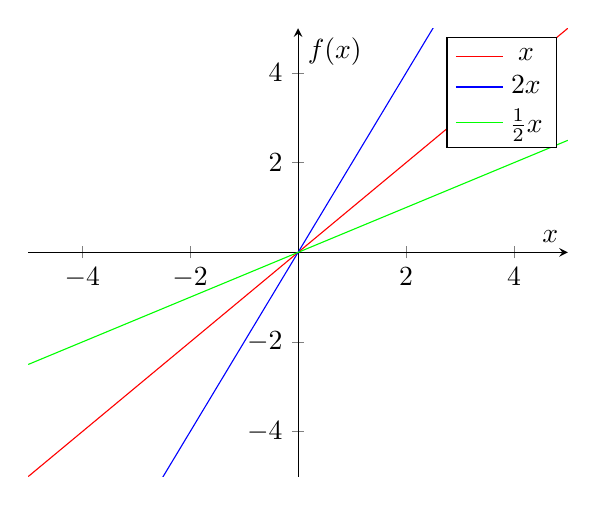
\begin{tikzpicture}
        \begin{axis}[
                axis lines = center,
                xlabel = $x$,
                ylabel = {$f(x)$},
                xmin=-5, xmax=5,
                ymin=-5, ymax=5,
            ]
            \addplot [
                domain=-5:5,
                samples=100,
                color=red,
            ]
            {x};
            \addlegendentry{$x$}
            \addplot [
                domain=-5:5,
                samples=100,
                color=blue,
            ]
            {2*x};
            \addlegendentry{$2x$}
            \addplot [
                domain=-5:5,
                samples=100,
                color=green,
            ]
            {0.5*x};
            \addlegendentry{$\frac{1}{2}x$}
        \end{axis}
    \end{tikzpicture}
\end{center}

\subsection{Funzione potenza}
$y = x^n$ con $n \in \mathbb{R}$\\
Strettamente crescente per $x\geq 0$, cioè:
\[
    0 \leq x_1 < x_2 \implies x_1^n < x_2^n
\]
(Ad esempio per $n = 2$ se $0\leq x_1 \leq x_2$ moltiplicando per $x_1$ e $x_2$ si ha $x_1^2 < x_1x_2$ e $x_1x_2 < x_2^2 \implies x_1^2 < x_2^2$) e quindi è invertibile e l'inversa è:
\[
    f^{-1}(x) = \sqrt[n]{x} = x^{\frac{1}{n}} \ \ \ x \geq 0
\]

\begin{center}
    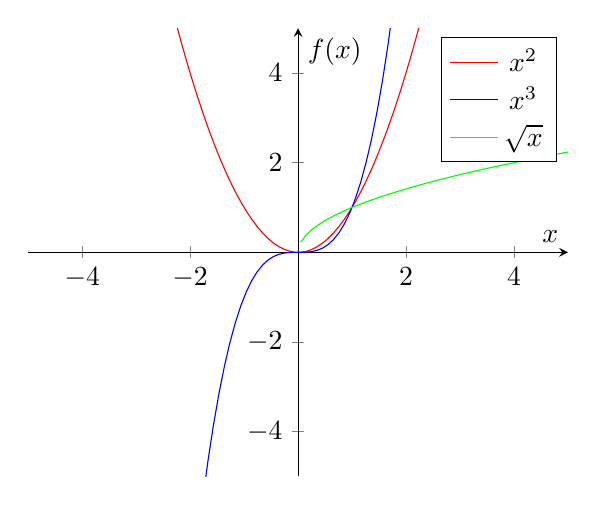
\begin{tikzpicture}
        \begin{axis}[
                axis lines = center,
                xlabel = $x$,
                ylabel = {$f(x)$},
                xmin=-5, xmax=5,
                ymin=-5, ymax=5,
            ]
            \addplot [
                domain=-5:5,
                samples=100,
                color=red,
            ]
            {x^2};
            \addlegendentry{$x^2$}
            \addplot [
                domain=-5:5,
                samples=100,
                color=blue,
            ]
            {x^3};
            \addlegendentry{$x^3$}
            \addplot [
                domain=-5:5,
                samples=100,
                color=green,
            ]
            {x^0.5};
            \addlegendentry{$\sqrt{x}$}
        \end{axis}
    \end{tikzpicture}
\end{center}

\subsection{Funzione esponenziale}
$f(x) = a^x$ con $a$ numero reale positivo, definita per ogni $x\in \mathbb{R}$
\begin{center}
    \begin{tikzpicture}
        \begin{axis}[
                axis lines = center,
                xlabel = $x$,
                ylabel = {$f(x)$},
                xmin=-5, xmax=5,
                ymin=-5, ymax=5,
            ]
            \addplot [
                domain=-5:5,
                samples=100,
                color=red,
            ]
            {e^x};
            \addplot [
                domain=-5:5,
                samples=100,
                color=blue,
            ]
            {e^-x};
            \addlegendentry{$e^x$}
            \addlegendentry{$e^{-x}$}
        \end{axis}
    \end{tikzpicture}
\end{center}
Se $a\neq 1$, allora la funzione esponenziale è invertibile, la funzione inversa è:

\subsection{Funzione logaritmo}
$f(x) = \log_a x$.
\[
    y = \log_a x \iff a^y = x
\]

\begin{center}
    \begin{tikzpicture}
        \begin{axis}[
                axis lines = center,
                xlabel = $x$,
                ylabel = {$f(x)$},
                xmin=-5, xmax=5,
                ymin=-5, ymax=5,
            ]
            \addplot [
                domain=0.01:5,
                samples=100,
                color=red,
            ]
            {ln(x)};
            \addplot [
                domain=-5:-0.01,
                samples=100,
                color=red,
            ]
            {ln(-x)};
            \addlegendentry{$\ln x$}
            \addlegendentry{$\ln -x$}
        \end{axis}
    \end{tikzpicture}
\end{center}

\subsection{Funzione valore assoluto}
\begin{itemize}
    \item $|x| \leq r \iff -r \leq x \leq r$
    \item $|x_1 + x_2| \leq |x_1| + |x_2| \ \ \ \forall x_1, x_2$
\end{itemize}
\begin{center}
    \begin{tikzpicture}
        \begin{axis}[
                axis lines = center,
                xlabel = $x$,
                ylabel = {$f(x)$},
                xmin=-5, xmax=5,
                ymin=-5, ymax=5,
            ]
            \addplot [
                domain=-5:5,
                samples=100,
                color=red,
            ]
            {abs(x)};
            \addlegendentry{$|x|$}
        \end{axis}
    \end{tikzpicture}
\end{center}

\subsection{Funzioni trigonometriche}
$y = \sin x, \cos x$
\begin{itemize}
    \item $-1 \leq \sin x \leq 1$ e $-1 \leq \cos x \leq 1$
    \item $\sin^2 x + \cos^2 x = 1$
\end{itemize}
\begin{center}
    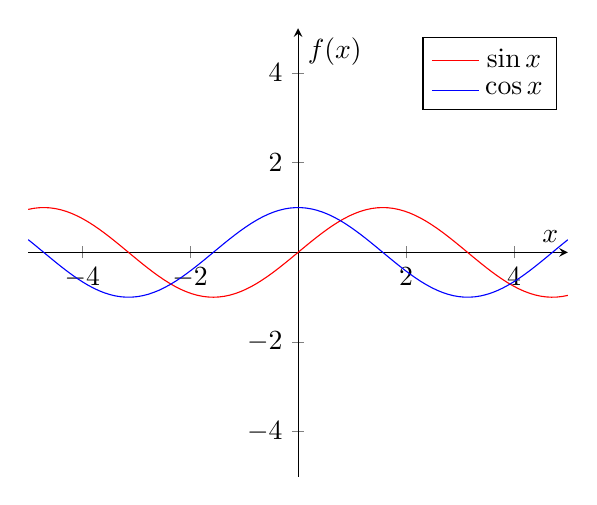
\begin{tikzpicture}
        \begin{axis}[
                axis lines = center,
                xlabel = $x$,
                ylabel = {$f(x)$},
                xmin=-5, xmax=5,
                ymin=-5, ymax=5,
            ]
            \addplot [
                domain=-5:5,
                samples=100,
                color=red,
            ]
            {sin(deg(x))};
            \addlegendentry{$\sin x$}
            \addplot [
                domain=-5:5,
                samples=100,
                color=blue,
            ]
            {cos(deg(x))};
            \addlegendentry{$\cos x$}
        \end{axis}
    \end{tikzpicture}
\end{center}
E' interessante vedere la combinazione di funzioni elementari.\\
Consideriamo la funzione $f(x) = \dfrac{\sin x}{x}$ definita per $\forall x \in \mathbb{R} \setminus \{0\}$.
E' una funzione \textbf{pari}, cioè $f(x) = f(-x) \ \ \ \forall x \in \text{ dominio}$, simmetrica rispetto all'asse $y$.\\
(\textbf{Dispari} se $f(x) = -f(-x)$, simmetrica rispetto all'origine).\\
\subsection{Esempio, Introduzione limiti}
\begin{itemize}
    \item $y = x$, $y = \sin x$ sono funzioni Dispari
    \item $y = \cos x$ è una funzione Pari
\end{itemize}
$f(x) = \dfrac{\sin x}{x}$ è una funzione pari, la disegniamo per $x \geq 0$.\\
Osserviamo che $-1 \leq \sin x \leq 1 \ \forall x \in \R$ e dividendo per x: $\implies -\dfrac{1}{x} \leq \dfrac{\sin x}{x} \leq \dfrac{1}{x} \ \ \ \forall x > 0$\\
\begin{center}
    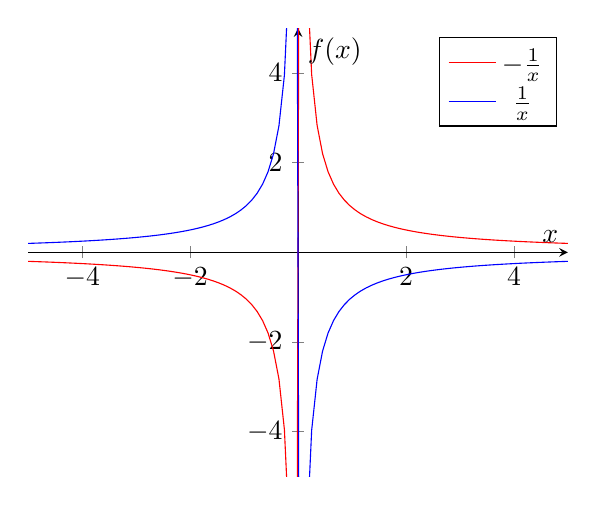
\begin{tikzpicture}
        \begin{axis}[
                axis lines = center,
                xlabel = $x$,
                ylabel = {$f(x)$},
                xmin=-5, xmax=5,
                ymin=-5, ymax=5,
            ]
            \addplot [
                domain=-5:5,
                samples=100,
                color=red,
            ]
            {1/x};
            \addplot [
                domain=-5:5,
                samples=100,
                color=blue,
            ]
            {-1/x};
            \addlegendentry{$-\frac{1}{x}$}
            \addlegendentry{$\frac{1}{x}$}

        \end{axis}
    \end{tikzpicture}
\end{center}
e $y = \dfrac{\sin x}{x}$ sarà compresa tra i due rami di iperbole per $x > 0$:
% plot only x > 0 zoom the space between the two branches

\begin{center}
    \begin{tikzpicture}
        \begin{axis}[
                axis lines = center,
                xlabel = $x$,
                ylabel = {$f(x)$},
                xmin=0, xmax=1.1,
                ymin=-5, ymax=5,
            ]
            \addplot [
                domain=0.01:5,
                samples=100,
                color=red,
            ]
            {1/x};
            \addplot [
                domain=0.01:5,
                samples=100,
                color=blue,
            ]
            {-1/x};
            \addlegendentry{$\frac{1}{x}$}
            \addlegendentry{$-\frac{1}{x}$}
        \end{axis}
    \end{tikzpicture}
\end{center}
per $x > 0$, $y = \dfrac{\sin x}{x}$ ha lo stesso segno di $\sin x$:
\begin{center}
    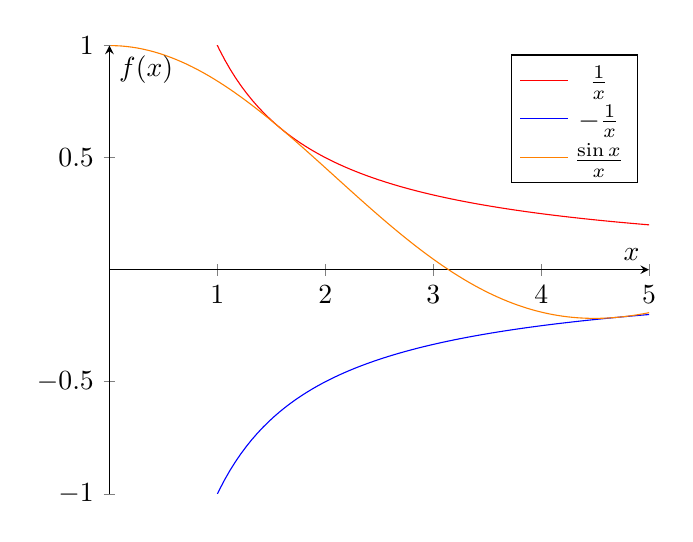
\begin{tikzpicture}
        \begin{axis}[
                axis lines = center,
                xlabel = $x$,
                ylabel = {$f(x)$},
                xmin=0, xmax=5,
                ymin=-1, ymax=1,
            ]
            \addplot [
                domain=0.01:5,
                samples=100,
                color=red,
            ]
            {1/x};
            \addplot [
                domain=0.01:5,
                samples=100,
                color=blue,
            ]
            {-1/x};

            \addplot [
                domain=0.01:5,
                samples=100,
                color=orange,
            ]
            {sin(deg(x))/x};

            \addlegendentry{$\frac{1}{x}$}
            \addlegendentry{$-\frac{1}{x}$}
            \addlegendentry{$\frac{\sin x}{x}$}
        \end{axis}
    \end{tikzpicture}
\end{center}
$x_n \to 0 \ \ \ f(x_n) \to \ ?$\\
Non è definita per $x = 0$. Cosa succede per $x \to 0$?\\
\begin{itemize}
    \item Tende a zero?
    \item Tende a $+\infty$?
    \item O tende a un valore intermedio?
\end{itemize}
Una formulazione rigorosa del comportamento di una funzione $f(x)$, per $x$ vicino ad un punto $x_0$,
in questo caso $x_0 = 0$, è quella di considerare una generica successione $x_n$ che converge ad $x_0$
($x_n$ è "vicino" ad $x_0$ se $n$ è grande) e la corrispondente successione $y_n$ costutuita dai valori assunti dalla funzione $f(x)$ ($y_n = f(x_n)$, $\forall n\in \mathbb{N}$).\\
Se $y_n = f(x_n)$ converge ad un numero $l$ (che è lo stesso $\forall x_n \to x_0$), allora si dice che $f(x)$ ammette limite
uguale a $l$ per $x \to x_0$.\\

Tornando all'esempio di $f(x) = \dfrac{\sin x}{x}$, calcolo
\[
    \lim_{x\to+\infty} f(x_n) = \lim_{x\to+\infty} \frac{\sin x_n}{x} = ?
\]
è il limite notevole per le successioni, che sappiamo valere $1$.\\
$\implies \lim_{x\to +\infty} \ f(x_n) = \lim_{x\to +\infty} \frac{\sin x_n}{x_n} = 1 \iff \lim_{x\to 0} \frac{\sin x}{x} = 1$\\
\begin{center}
    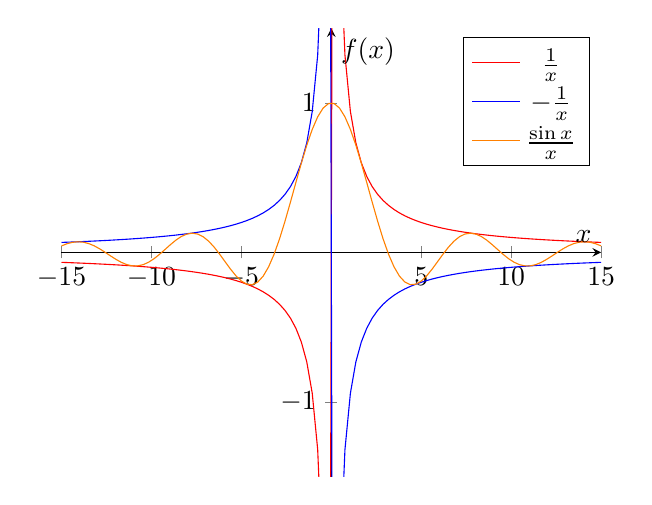
\begin{tikzpicture}
        \begin{axis}[
                axis lines = center,
                xlabel = $x$,
                ylabel = {$f(x)$},
                xmin=-15, xmax=15,
                ymin=-1.5, ymax=1.5,
            ]
            \addplot [
                domain=-15:15,
                samples=100,
                color=red,
            ]
            {1/x};
            \addplot [
                domain=-15:15,
                samples=100,
                color=blue,
            ]
            {-1/x};

            \addplot [
                domain=-15:15,
                samples=100,
                color=orange,
            ]
            {sin(deg(x))/x};

            \addlegendentry{$\frac{1}{x}$}
            \addlegendentry{$-\frac{1}{x}$}
            \addlegendentry{$\frac{\sin x}{x}$}
        \end{axis}
    \end{tikzpicture}
\end{center}

\subsection{Definizione di limite}
Sia $A$ un intervallo, o unione finita di intervalli e sia $x_0 \in A$ (anche
all'estremo).\\ Si dice che $f(x)$ ha limite uguale ed $l$ (tende o converge ad
$l$) per $x \to x_0$ se qualunque sia la successione $x_n \to x_0$, con $x_n\in
    A$ e $x_n \neq x_0 \ \forall n$ risulta che $f(x_n) \to l$.\\ Si dimostra che
questa definizione è equivalente alla seguente:
\[
    \lim_{x\to x_0} f(x) = l \iff \forall \varepsilon > 0 \ \exists \delta > 0 \ : \ |f(x) - l| < \varepsilon \ \ \ \forall x \in A \ : \ 0 \neq |x - x_0| < \delta
\]

\subsection{Teorema del legame tra limiti di funzioni e limiti di successioni}
Le seguenti relazioni sono fra loro equivalenti ($x_0, l\in\R$).
\begin{itemize}
    \item $\forall x_n \to x_0 \ x_n \in A \setminus \{x_0\} \ \forall n\in \mathbb{N} \implies f(x_n) \to l$
    \item $\forall\varepsilon>0 \ \exists\delta>0 \ : \ x\in A, \ 0\neq |x-x_0|<\delta \implies |f(x)-l|<\varepsilon$
\end{itemize}
Valgono anche le definizioni con i limiti infiniti:
\begin{itemize}
    \item $\lim_{x\to x_0} f(x) = +\infty \iff \forall x_n \to x_0 \ x_n \in A \setminus \{x_0\} \ \forall n \in \mathbb{N} \implies f(x_n) \to +\infty /iff \forall M > 0 \ \exists \delta > 0 \ : f(x) > M \ \ \ \forall x \in A \ : \ 0 \neq |x - x_0| < \delta$
    \item $\lim_{x\to x_o} f(x) = l \iff \forall x_n\to+\infty, \ x_n\in A, \ \forall n \in \mathbb{N} \implies f(x_n) \to l \iff \forall \varepsilon > 0 \ \exists k \ : \ |f(x) - l| < \varepsilon \ \ \ \forall x \in A \ : \ x > k$
    \item $\lim_{x\to+\infty} f(x) = +\infty \iff \forall x_n \to +\infty \ x_n \in A \ \forall n \in \mathbb{N} \implies f(x_n) \to +\infty \iff \forall M > 0 \ \exists k \ : \ f(x) > M \ \ \ \forall x \in A \ : \ x > k$
\end{itemize}
\textbf{Osservazione:} è utile considerare il \textbf{limite destro $x\to x_0^+$} e il \textbf{limite sinistro $x\to x_0^-$}, quando ci si avvicina al punto $x_0$ per valori di $x\in A$ rispettivamente solo maggiori di $x_0$, o solo minori.
\begin{itemize}
    \item $\lim_{x\to x_0^+} f(x) = l \iff \forall\varepsilon > 0,\delta > 0 \ : \ |f(x)-l|<\varepsilon \ \ \ \forall x \in A \ : \ 0 < x - x_0 < \delta$
    \item $\lim_{x\to x_0^-} f(x) = l \iff \forall\varepsilon > 0,\delta > 0 \ : \ |f(x)-l|<\varepsilon \ \ \ \forall x \in A \ : \ -\delta < x - x_0 < 0$
\end{itemize}

\subsection{Operazioni con i limiti di funzioni}
Il limite della somma, differenza, prodotto, quoziente, di due funzioni è
rispettivamente uguale alla somma, differenza, prodotto, quazionete (se il
denominatore è diverso da zero) dei due limiti, purchè non sia una delle forme
indeterminate.

\subsection{Limiti Notevoli}
Valgono i limiti notevoli visti per le successioni:
\begin{itemize}
    \item $\lim_{x\to 0} a^x = \begin{cases}
                  +\infty & \text{se } a > 1     \\
                  0       & \text{se } 0 < a < 1
              \end{cases}$\\In particolare $\lim_{x\to+\infty} e^x = +\infty$ e $\lim_{x\to-\infty} e^x = 0$
    \item $\lim_{x\to +\infty} \ln x = +\infty$ e $\lim_{x\to 0^+} \ln x = -\infty$
    \item $\lim_{x\to\pm\infty} (1+\frac{1}{x})^x = e$
    \item $\lim_{x\to\pm\infty} (1+\frac{b}{x})^x = e^b \ \ \ \forall b\in\R$\\ In generale $(1+f(x))^{\frac{1}{f(x)}} \to e \ \ \ \text{per } f(x)\to 0$
    \item $\lim_{x\to0} \dfrac{\sin x}{x} = 1$
    \item $\lim_{x\to0} \dfrac{1-\cos x}{x^2} = \frac{1}{2}$
    \item $\lim_{x\to0} \dfrac{1-\cos x}{x} = 0$
\end{itemize}

\subsection{Limiti di funzioni composte}
Siano $g: x \to y$ e $f: y \to \R$ due funzioni, tali che:
\[
    \lim_{x\to x_0} g(x) = y_0 \text{ e } \lim_{y\to y_0} f(y) = l
\]
ed esiste $\delta > 0$ tale che risulti $g(x) \neq y_0 \forall x\neq x_0$
dell'intervallo $(x_0 - \delta, x_0 + \delta)$, allora:
\[
    f \circ g: x \to \R \ \ \ \left[ f \circ g \right] (x) = f(g(x))
\]
si ha:
\[
    \lim_{x\to x_0} f(g(x)) = l
\]
segue che:
\[
    \lim_{x\to x_0} f(g(x)) = \lim_{y\to y_0} f(y) = l
\]
\textbf{Esempio:} Applichiamo il precedente risultato:\\
$\lim_{x\to\pm\infty} x\log(1+\frac{1}{x}) = 1$\\
Si può scrivere anche $1+y = t \implies \lim_{t\to 1} \dfrac{\log t}{t-1} = 1$\\

\end{document}